\documentclass[UTF8,11pt,a4paper]{ctexart}
\usepackage[margin=2.1cm]{geometry}
\usepackage{amsmath,amssymb,booktabs,longtable,tabularx,array,multirow}
\usepackage{graphicx,float,caption,subcaption,xcolor,hyperref,enumitem}
\usepackage{siunitx}
\usepackage{fancyhdr}
\hypersetup{colorlinks=true,linkcolor=black,citecolor=black,urlcolor=blue!55!black}
\setlength{\parindent}{2em}
\setlength{\parskip}{0.15em}
\renewcommand{\arraystretch}{1.18}
\pagestyle{fancy}
\setlength{\headheight}{14pt}
\fancyhf{}
\fancyhead[C]{2025 MCM Problem C：奥运奖牌榜预测}
\fancyfoot[C]{\thepage}

\newcommand{\E}{\mathbb{E}}
\newcommand{\R}{\mathbb{R}}
\newcommand{\keywords}[1]{\par\noindent\textbf{关键词：}#1}

\title{从上一届成绩到项目机会：\newline 2028 年奥运奖牌榜的收缩预测与项目跃升识别}
\author{正式竞赛长稿盲测（仅使用官方题面与所给数据）}
\date{2026 年 8 月}

\begin{document}
\maketitle

\begin{abstract}
题目提供了历届奖牌榜、运动员、主办地和比赛项目数据，要求预测 2028 年奖牌榜，并讨论首枚奖牌、比赛项目和“伟大教练”可能造成的变化。数据合并后有两个口径不能直接沿用：团队项目会把一枚奖牌重复记在多名运动员名下；题面所述项目表应含 2028 年，而本地附件的最后一列实际为 2024 年。本文以官方奖牌表作为国家总牌数和金牌数的目标值，运动员表只用于参赛规模与分项目归属；2028 年总项目数先按 2024 年结构处理，新增项目另作边际情景。

对总奖牌和金牌数，我们分别比较上一届成绩、含东道主修正的基线、对数岭回归、Poisson 梯度提升和随机森林。按 2008--2024 年逐届向前滚动验证，单独增加复杂度并未稳定改善误差；将东道主修正基线与随机森林各取一半后，全体国家误差与奖牌榜前 20 名误差取得较好折中。经全球奖牌总量校准，模型预测美国在 2028 年获得约 124.27 枚奖牌，其中金牌 43.79 枚；中国约 88.47 枚，其中金牌 38.86 枚。法国退出主场周期后总牌数回落至约 54.30 枚，加拿大、德国和日本的总牌数有小幅上升。

对于尚未获牌的国家，按历届参赛人数、项目数、参赛项目条目和参赛届数建立首牌 Logistic 模型。类别平衡训练提高了排序能力，但会抬高概率，因此再按滚动验证中的实际首牌率校准截距。2028 年预计约有 5.08 个国家取得首枚奖牌，90\% 计数区间为 2--9 个；黎巴嫩、南苏丹和巴勒斯坦列在当前候选前部。

运动员数据没有教练姓名，故不能由附件直接识别某位教练的因果效应。本文先控制既往奖牌、参赛人数、项目条目和东道主身份，再把同一国家--项目连续两届的正超额残差记为“教练型跃升候选”。中国体操、英国自行车和荷兰田径等历史片段进入候选集。进一步以近两届参赛规模固定、项目奖牌转化率提升至同项目上四分位为有限情景，建议德国关注田径、西班牙关注水上项目、埃及关注击剑，估计增量分别约为 4.10、4.07 和 3.56 枚。该数值表示可观测的能力缺口，不等同于教练的净因果贡献。

\keywords{奥运奖牌预测；滚动验证；收缩模型；首枚奖牌；项目机会；异常跃升}
\end{abstract}

\phantomsection\label{mcm-body-start}
\section{问题重述}

历届奥运会的奖牌数既受一国已有竞技基础影响，也会随主办地、参赛规模和项目设置变化。题目要求由所给数据完成四项工作：预测各国 2028 年金牌数和总奖牌数并给出区间；估计尚未获牌国家在下一届首次获牌的可能性；说明项目设置对不同国家的影响；从历史跃升中寻找可能的“伟大教练”效应，并为三个国家给出投资建议。模型还应给出可衡量的误差与不确定性，而不能只排出一个确定名次。

这四项任务共用同一历史面板，但对象并不相同。国家级预测以一国一届为样本；项目影响与教练型跃升需要把奖牌拆到国家--项目；首牌问题只保留预测时点以前从未获牌的代表团。若把三种样本单位混在同一张表中，团队项目的多人记录和国家名称的历届变化会同时进入目标值，后续误差将无法解释。

\section{问题分析：数据口径与模型接口}

\subsection{附件实际提供的信息}

运动员表共有 252565 行，一行代表某名运动员在某一项目中的参赛结果；奖牌表共有 1435 行，一行代表一个国家在某届奥运会的奖牌汇总。前者适合统计参赛人数、覆盖项目和项目归属，后者才是国家级预测的目标。以全部历史为例，运动员表中有 38818 行获牌记录，按“年份--NOC--项目--小项--奖牌类型”去重后只剩 18159 条，说明团队项目若按运动员行计数，会把一枚奖牌重复记给多人。

另一个差异来自项目表。题面说明项目数据覆盖到 2032 年，但本地压缩包实际只有 1896--2024 年各列。本文不根据上下文补造 2028 项目数：基准预测保持 2024 年的 329 个项目结构；当某项目新增或减少一枚奖牌时，再用国家在该项目中的近期份额计算边际变化。这样，项目数据缺口不会被隐藏在模型输入中。

\begin{table}[H]
\centering
\caption{四张主表在模型中的角色}
\label{tab:data-role}
\begin{tabularx}{\textwidth}{p{3.2cm}p{2.0cm}X X}
\toprule
数据表 & 样本单位 & 本文使用的字段 & 不直接承担的任务\\
\midrule
奖牌榜 & 国家--届次 & 金、银、铜、总牌数 & 不用于项目归属\\
运动员 & 运动员记录 & NOC、年份、项目、小项、奖牌 & 不按原始获牌行汇总国家总牌数\\
主办地 & 届次 & 主办国家 & 不把主场后所有变化都归为东道主效应\\
项目表 & 项目--届次 & 2024 年项目数与历史变化 & 不声称附件已给出 2028 精确项目表\\
\bottomrule
\end{tabularx}
\end{table}

\subsection{记录粒度、去重键与目标重建}

国家奖牌榜和运动员表的行含义不同，不能先把两张表按年份连接后再求和。本文先把运动员表中的项目名称规范到统一的 \texttt{SportC}，再建立项目层记录
\begin{equation}
\mathcal{R}=\{(y,n,s,e,m):y\text{ 为届次},n\text{ 为 NOC},s\text{ 为规范化项目},e\text{ 为小项},m\text{ 为奖牌类型}\}.
\end{equation}
在同一组键下只保留一条记录，并令
\begin{equation}
M_{n,s,y}=\sum_{e,m}\mathbf{1}\{(y,n,s,e,m)\in\mathcal{R}\}.
\end{equation}
这样做的含义是“一国在一个小项中获得一种奖牌记一枚”，而不是“每名运动员获得的奖牌都相加”。252565 行运动员记录中，38818 行带有奖牌标记；按上述五元键去重后得到 18159 条项目奖牌记录。这个数量差不是清洗时删掉了有效奖牌，而是团队小项的多人记录被还原为一个项目结果。

国家级目标不从 $M_{n,s,y}$ 反推，而是直接读取官方奖牌榜。代码按届次维护国家名称到 NOC 的映射：先使用当届可确定的官方标签，再处理历史别名和特殊代表团；若某个名称只在运动员表中出现而官方目标为零，则保留其项目归属，但不把它追加到国家总牌目标。2024 年韩国、捷克、伊朗、土耳其和香港经逐届映射后分别恢复为 32、5、12、8 和 4 枚总牌，这五个值也作为合并后的回归检查点。

\begin{table}[H]
\centering
\caption{目标表与项目表的连接检查}
\label{tab:join-check}
\small
\begin{tabularx}{\textwidth}{p{2.2cm}p{3.4cm}p{3.0cm}X}
\toprule
检查项 & 使用的键或口径 & 结果 & 作用\\
\midrule
国家目标 & 届次--NOC--总牌/金牌 & 2024 年总牌和为 1039、金牌和为 328 & 确定预测校准总量\\
项目归属 & 届次--NOC--规范化项目--小项--奖牌 & 去重后 18159 条 & 防止团队项目重复计数\\
国家名称 & 当届官方名称到 NOC 的映射 & 5 个易混名称通过检查 & 保持跨届特征连续\\
零目标检查 & 运动员有牌而官方目标为零的普通国家 & 数量为 0 & 检查映射是否漏牌\\
\bottomrule
\end{tabularx}
\end{table}

\subsection{国家名称跨届映射与特殊代表团}

同一代表团在不同年份的显示名称并不总是一致。实际实现把映射表按年份保存，而不是把一个固定的名称替换表套到全部历史。这样可以分别处理名称变化、分裂或合并，以及 AIN、难民队等不应进入“国家首牌候选”的特殊记录。对于项目情景，特殊代表团仍可以保留作历史份额计算；对于国家级 2028 预测，则只输出可以与题面国家清单对应的 NOC。

这一步也决定了特征的缺失值含义。某国在某届没有运动员行，不等于它“参赛人数为零且从未参赛”；只有在该届确实出现在参赛表后，才把 $A_{i,t}$、$S_{i,t}$ 和 $E_{i,t}$ 置为相应统计量。历史面板补齐的是可预测国家--届次组合，补齐后的零奖牌是目标值，不是把缺席国家伪装成零表现。这个区别在首牌模型中尤其重要：候选集必须是预测时点实际参赛、此前累计奖牌为零的代表团。

\subsection{时间边界与无未来信息}

国家级预测使用 1896--2024 年可重建的届次面板，但每个验证点只看此前数据。对 2008 年的验证，训练集在 2004 年结束；对 2012、2016、2020 和 2024 年依次向前移动。2028 年预测只用到 2024 年，项目表的最后可用列也止于 2024 年。由此，题目中提到的 2028 项目表缺列不会以“未来字段”形式泄漏进特征。

代码中所有滚动特征先按国家和年份排序，再用 \texttt{shift(1)} 取得上一届值。最近三届加权均值的权重固定为 0.2、0.3、0.5，权重最大的届次是上一届；若历史不足三届，则按已有届次重新归一化。参赛人数、项目数和小项条目也使用同样的滞后口径。每次预测完成后才把当届结果写入下一届的训练面板，这使验证误差可以解释为真正的“向前预测”误差。

\subsection{为什么不直接选一个复杂模型}

奖牌榜的多数国家长期为零或个位数，少数强国占据较大份额。在这种分布下，一个模型即使把强国预测错十余枚，也可能因为正确预测了大量零值而取得较小的总体平均绝对误差。因此模型选择同时看两种口径：全部参赛国的 MAE，以及每届实际总牌数前 20 名的 MAE。前者检查整体，后者约束奖牌榜主体。

上一届成绩是必须保留的基线。若历史表现没有明显变化，它本身已经包含训练体系、人口和长期投入等难以在附件中逐项观测的因素。东道主身份却会造成局部变化：历届主办国的增量有时很大，退出主场周期时又不能继续保留同样加成。由此，本文先在基线上估计东道主修正，再让随机森林只负责吸收既往趋势、参赛规模和项目机会中未被基线表达的部分；两者各占一半，避免树模型把短期波动全部外推到下一届。

首牌问题的正样本更少。平衡类别权重能帮助模型识别潜在国家，却会把输出概率整体推高。故分类器首先用于排序，概率还要回到历届滚动预测中按真实首牌发生率校准。至于“伟大教练”，附件没有教练姓名和任职年份，直接把一次奖牌增加写成教练效应没有数据依据。可做的是先找出控制已有条件后仍连续超额的项目，再把它们列为需要外部教练履历复核的候选。

\section{模型假设}

\begin{enumerate}[label=\arabic*)]
\item 同一届同一 NOC、规范化项目、小项和奖牌类型对应一枚项目奖牌；同一团队的多名运动员记录不重复计奖。
\item 2028 年基准情景沿用 2024 年项目总量。项目增减只在情景分析中改变，不进入基准点预测。
\item 东道主加成取预测时点以前历届主办国相对于按项目总量缩放基线的中位残差；离开主场的下一届扣除同一加成。
\item 模型只在所给历史数据范围内解释。连续正残差可标记项目跃升，但没有教练履历时不作教练因果判定。
\item 首牌模型把 AIN、难民队和历史混合代表队等非国家代表团排除在候选数量之外。
\end{enumerate}

\section{符号说明}

\subsection{主要符号}

\begin{table}[H]
\centering
\caption{主要符号}
\label{tab:symbols}
\begin{tabular}{cll}
\toprule
符号 & 含义 & 单位或范围\\
\midrule
$Y^{T}_{i,t}$ & 国家 $i$ 在第 $t$ 届的总奖牌数 & 枚\\
$Y^{G}_{i,t}$ & 国家 $i$ 在第 $t$ 届的金牌数 & 枚\\
$A_{i,t}$ & 参赛运动员人数 & 人\\
$S_{i,t}$ & 覆盖的规范化项目数 & 项\\
$E_{i,t}$ & 参加的小项条目数 & 项\\
$H_{i,t}$ & 是否为东道主 & $0/1$\\
$O_{i,t}$ & 近期项目机会得分 & 非负实数\\
$p_{i,t}$ & 从未获牌国家首次获牌概率 & $[0,1]$\\
$M_{i,s,t}$ & 国家 $i$ 在项目 $s$、届次 $t$ 的奖牌数 & 枚\\
$r_{i,s,t}$ & 项目模型的超额残差 & 枚\\
\bottomrule
\end{tabular}
\end{table}

\subsection{特征字典与可复算接口}

国家级特征不是把运动员表的 252565 行直接喂给模型，而是先压缩到国家--届次。最终进入随机森林的 17 个变量可按来源分为四组。历史组包括上一届总牌、上一届金牌、最近三届加权总牌和金牌、总牌与金牌的近两届变化；参赛组包括上一届运动员人数、规范化项目数、小项条目数、累计参赛届数和累计获牌届数；主办与项目组包括主办标记、离开主场标记、当届项目总数、上一届项目总数、项目总量缩放比和项目机会得分。对总牌和金牌分别建模，目标列不出现在同届特征中。

\begin{longtable}{p{3.4cm}p{4.4cm}p{7.0cm}}
\caption{国家级特征字典及其在模型中的用途}\label{tab:feature-dictionary}\\
\toprule
特征组 & 字段 & 计算口径与用途\\
\midrule
\endfirsthead
\toprule
特征组 & 字段 & 计算口径与用途\\
\midrule
\endhead
\midrule
\multicolumn{3}{r}{续下页}\\
\endfoot
\bottomrule
\endlastfoot
历史 & \path{lag_total}, \path{lag_gold} & 上一届官方总牌和金牌，保留最直接的惯性信息。\\
历史 & \path{ewm_total}, \path{ewm_gold} & 最近三届按 0.2、0.3、0.5 加权，降低单届偶然波动。\\
历史 & \path{trend_total}, \path{trend_gold} & 最近两届变化量，记录上升或回落方向。\\
参赛 & \path{lag_athletes} & 上一届去重运动员人数，作为代表团规模代理。\\
参赛 & \path{lag_sports}, \path{lag_event_entries} & 上一届覆盖项目和小项条目，表示可进入的比赛面。\\
积累 & \path{participation_editions} & 预测时点以前出现过的届数，区分新进入者与长期参赛者。\\
积累 & \path{medal_editions} & 预测时点以前获牌的届数，反映稳定奖牌基础。\\
主办 & \path{host}, \path{post_host} & 当届东道主与离开主场的状态，供式\eqref{eq:hostbase}调整。\\
项目 & \path{event_total}, \path{lag_event_total} & 当届和上一届全球小项数，用于缩放基线。\\
项目 & \path{event_scale} & 当届项目总量与上一届的比值，供持续性基线缩放。\\
机会 & \path{opportunity} & 式\eqref{eq:opportunity}定义的近期优势项目份额。\\
\end{longtable}

这些字段有两个接口约束。第一，国家表的历史统计和项目表的项目份额必须在同一个年份截断，不能先用 2024 年项目份额回填 2012 年的训练行。第二，项目机会只作为国家层面的解释变量，不把它拆成“已获得奖牌”；实际奖牌仍由官方国家目标提供。特征表生成后，代码写出 \texttt{model\_panel.csv}，其中每一行都能追溯到国家、届次和目标值，便于重新检查滞后是否错位。

\subsection{训练样本的逐届构造}

训练面板的构造顺序固定为：
\begin{enumerate}[label=(\alph*)]
\item 按年份清理国家标签，并从运动员表得到国家--届次的参赛规模和项目归属；
\item 从官方奖牌榜取得国家总牌和金牌目标，填入同一届次索引；
\item 对每个国家按年份排序，计算上一届、最近三届和累计变量；
\item 把主办地和当届项目数合并，生成主场状态与项目机会；
\item 在目标届次前截断面板，训练候选模型并记录验证误差；
\item 预测结束后再把该届目标写入下一届的历史窗口。
\end{enumerate}
这六步看似只是数据处理，但它们决定了“上一届成绩”到底是哪一届，也决定了 2020 年特殊比赛安排是否被当成新的项目结构。遇到缺失的参赛规模，代码不从奖牌榜倒推人数；遇到项目名称无法规范化的行，则保留原始行供审查并不进入项目份额汇总。对 2028 年，最后一步只延伸特征，不延伸未经附件给出的项目列。

\section{分问题模型建立与求解}

\phantomsection\label{mcm-q1-start}
\subsection{奖牌数预测模型}

\subsubsection{特征随届次向前构造}

对每个国家--届次样本，只使用该届以前的信息。记最近一届总牌和金牌为 $L^T_{i,t}$、$L^G_{i,t}$，最近三届按 $0.2,0.3,0.5$ 加权得到 $W^T_{i,t}$、$W^G_{i,t}$；另记录最近两届的变化量、上届参赛人数、覆盖项目数、小项条目数、累计参赛届数和累计获牌届数。项目机会得分写为
\begin{equation}
O_{i,t}=\sum_s N_{s,t}\frac{\sum_{\tau\in\mathcal{T}_3}M_{i,s,\tau}}
{\sum_j\sum_{\tau\in\mathcal{T}_3}M_{j,s,\tau}},
\label{eq:opportunity}
\end{equation}
其中 $N_{s,t}$ 是项目 $s$ 的奖牌小项数，$\mathcal{T}_3$ 为此前三届。该量不是奖牌预测值；它只表示当前项目结构把多少机会放在一国近期较强的项目上。

\subsubsection{东道主状态校正}

若当前届项目总数相对上一届变化，先将上一届奖牌数按比例缩放：
\begin{equation}
B^q_{i,t}=L^q_{i,t}\frac{N_t}{N_{t-1}},\qquad q\in\{T,G\}.
\end{equation}
在训练窗口内，对此前所有主办国计算 $Y^q_{i,t}-B^q_{i,t}$，取中位数为 $b^q_t$。于是
\begin{equation}
\widetilde{B}^q_{i,t}=\max\left\{0,
B^q_{i,t}+b^q_t H_{i,t}-b^q_t H_{i,t-1}\right\}.
\label{eq:hostbase}
\end{equation}
第二项描述主场加成，第三项处理离开主场后的回落。这里没有把主办国每一次增长都写成固定比例；中位残差限制了北京、东京等高增量届次对估计的支配。

\subsubsection{收缩预测的两部分}

除式\eqref{eq:hostbase}外，使用同一训练窗口分别拟合对数岭回归、Poisson 梯度提升和随机森林。随机森林输入上述 17 个历史特征，输出非负奖牌数。初步试算表明，单独使用树模型对少数强国有改善，但在全体国家上容易把短期起伏放大；只使用基线则难以给出国家间的差异变化。最终取
\begin{equation}
\widehat{Y}^q_{i,t}=0.5\widetilde{B}^q_{i,t}+0.5F^q(\boldsymbol{x}_{i,t}),
\label{eq:blend}
\end{equation}
其中 $F^q$ 为随机森林预测。该权重不是由 2028 结果反推，而是在滚动验证中与 $0.25/0.75$、$0.5/0.5$ 等候选同口径比较后确定。

各国点预测最后按同一常数缩放，使总奖牌数和金牌数分别回到 2024 项目情景的 1039 枚和 328 枚；逐国再检查 $0\leq \widehat{Y}^G_{i,t}\leq \widehat{Y}^T_{i,t}$。区间由 2008--2024 年滚动预测残差的 5\% 与 95\% 分位数给出，并按预测规模分箱。它表示历史同口径误差范围，不是参数模型下的正态置信区间。

\subsubsection{滚动验证}

每次验证只用目标届以前的样本训练，再预测 2008、2012、2016、2020 和 2024。图\ref{fig:validation}给出各模型的平均 MAE。复杂模型没有因为名称更复杂而自动胜出：总奖牌的上一届基线 MAE 为 1.47，随机森林为 1.54；加入东道主修正后再与随机森林收缩，最终方案 MAE 为 1.44。金牌的最终方案 MAE 为 0.63，低于上一届基线的 0.67。

\begin{figure}[H]
\centering
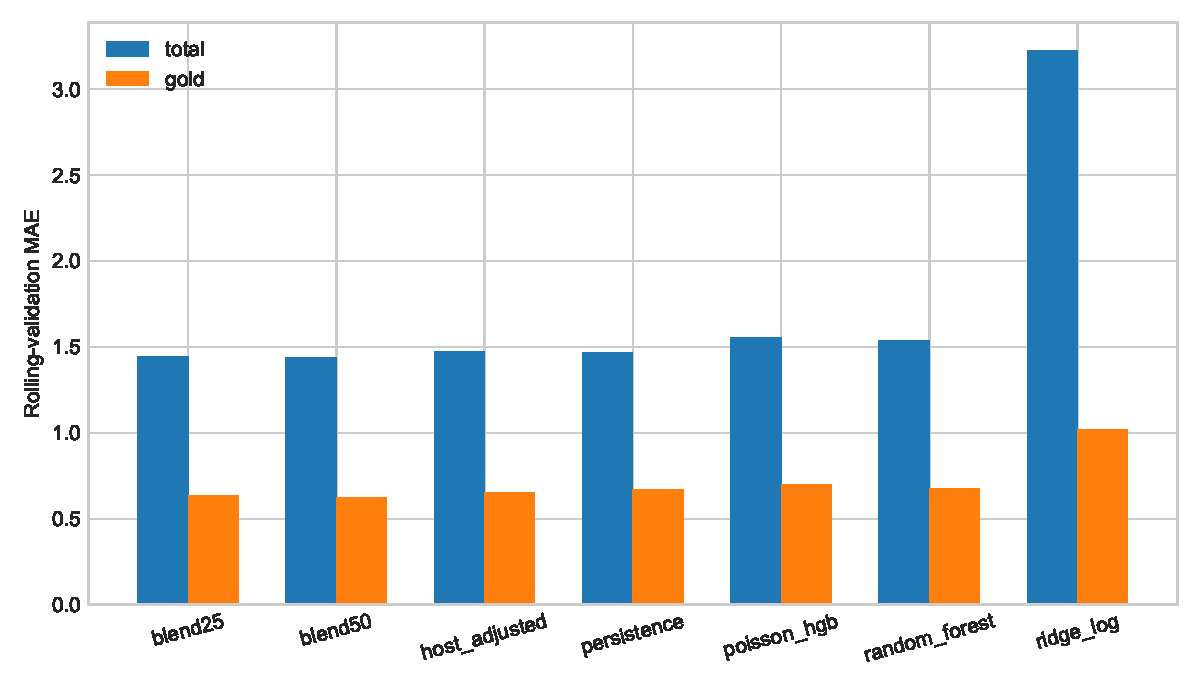
\includegraphics[width=0.78\textwidth]{figures/validation_mae.pdf}
\caption{2008--2024 年逐届滚动验证的平均绝对误差}
\label{fig:validation}
\end{figure}

\subsubsection{验证中的逐届差异}

平均 MAE 只给出一个汇总数，不能说明模型在哪一届失去优势。图\ref{fig:rolling-year}把最终收缩方案与上一届基线按验证届次展开。2020 年所有方案的误差都抬高，原因是比赛延期、代表团规模和项目安排同时发生变化；在这一届，收缩方案的总牌 MAE 为 1.858，仍低于上一届基线的 1.913。2012 年 25\% 收缩的总牌误差最低，但 2020 年和全期平均更支持 50\% 收缩，所以没有用单一届次的最好值替代滚动平均。

\begin{figure}[H]
\centering
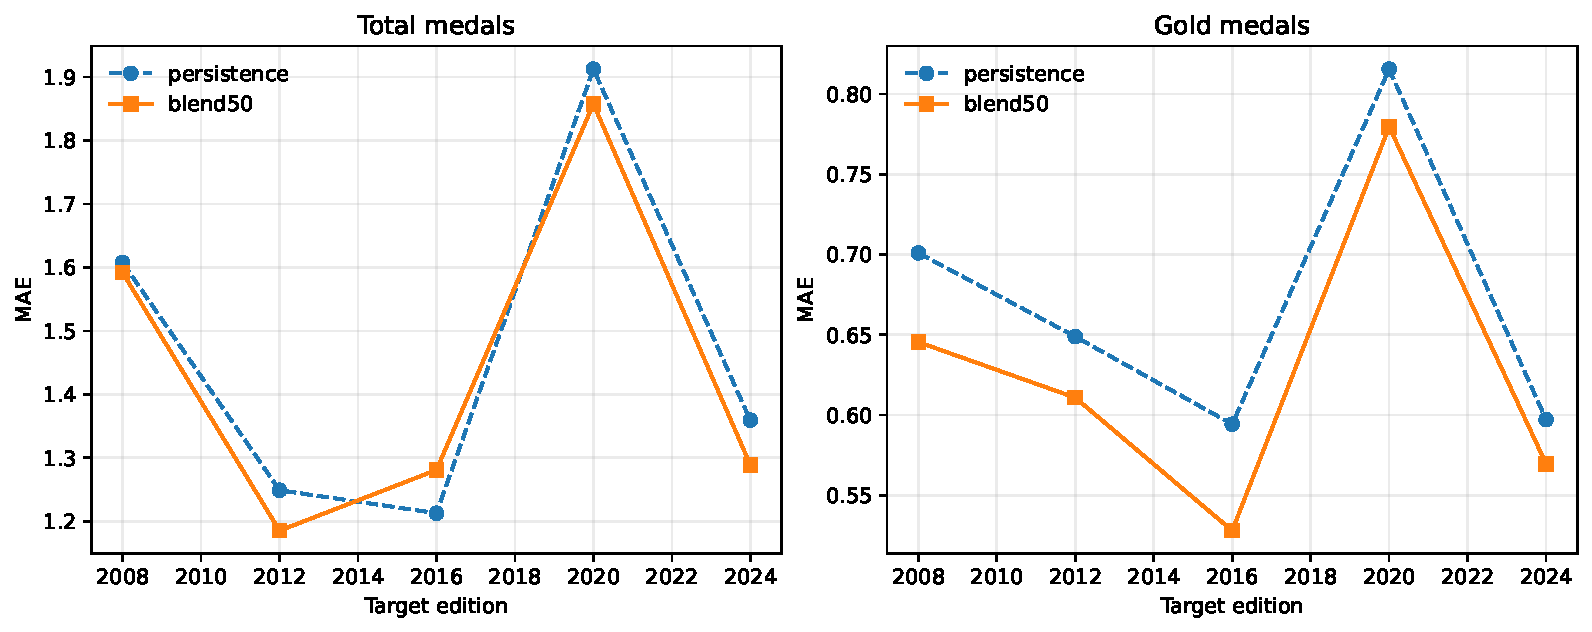
\includegraphics[width=0.79\textwidth]{figures/rolling_by_year.pdf}
\caption{最终收缩方案与上一届基线的逐届 MAE}
\label{fig:rolling-year}
\end{figure}

\begin{table}[H]
\centering
\caption{总牌预测的逐届误差（部分模型）}
\label{tab:rolling-detail}
\small
\begin{tabular}{lrrrrrr}
\toprule
验证届次 & 持续性 MAE & 主场基线 MAE & 25\% 收缩 & 50\% 收缩 & 50\% 前20名 & 50\% RMSE\\
\midrule
2008 & 1.608 & 1.581 & 1.573 & 1.592 & 8.842 & 4.121\\
2012 & 1.249 & 1.173 & 1.149 & 1.185 & 4.818 & 2.506\\
2016 & 1.213 & 1.329 & 1.295 & 1.281 & 6.510 & 3.013\\
2020 & 1.913 & 2.000 & 1.924 & 1.858 & 9.741 & 5.799\\
2024 & 1.359 & 1.290 & 1.276 & 1.289 & 5.680 & 2.923\\
\bottomrule
\end{tabular}
\end{table}

表中前 20 名误差使用该届真实总牌排序后再计算，因而不是把 20 个国家固定成 2028 年的前 20 名。2020 年的整体抬升和 2012 年的局部下降都被保留在选择样本里，没有在误差汇总前删除异常届次。这样得到的 50\% 方案不是“每届都最好”，而是在五个时间切片上把强国和长尾国家的误差放在同一个取舍中。

\subsubsection{三类模型的实现约束}

对数岭回归先对目标加一取对数，反变换后截断到非负；Poisson 梯度提升使用最大深度 3、180 棵迭代树、学习率 0.06、叶节点最少 15 个样本和 $L_2$ 正则 1.5；随机森林使用 17 个输入列、每次分裂抽取 0.8 的特征、固定随机种子 20250814，并以非负输出作为结果。持续性模型和主场基线不经过训练，分别作为“上一届不变”和“上一届按项目总量缩放并加主场残差”的可解释参照。

训练时没有把预测结果再作为下一届的观测输入。对于每个验证届次，代码保存逐国预测、实际值、误差和是否属于当届总牌前 20 名；\texttt{rolling\_predictions.csv}因而可以回答“某一国在哪一届被高估或低估”，而不仅是重算平均数。最终选模指标为
\begin{equation}
J_k=0.35\frac{\operatorname{MAE}_k}{\operatorname{MAE}_{\rm pers}}
 +0.65\frac{\operatorname{MAE}^{20}_k}{\operatorname{MAE}^{20}_{\rm pers}},
\end{equation}
其中上标 20 表示当届真实前 20 名。只有当候选方案相对持续性基线的综合值低于 0.98 时，复杂模型才可以取代持续性方案；本题总牌和金牌的赢家均为 \texttt{blend50}。

\subsubsection{从目标变换到非负输出}

对数岭回归的作用是提供一个方向明确的线性参照。令 $u_{i,t}=\log(1+Y_{i,t})$，在标准化后的特征上求解
\begin{equation}
\min_{\boldsymbol\beta}\sum_{i,t}(u_{i,t}-\beta_0-\boldsymbol{x}_{i,t}^{\mathsf T}\boldsymbol\beta)^2
 +\lambda\|\boldsymbol\beta\|_2^2,
\end{equation}
预测后用 $\exp(\widehat u)-1$ 反变换。这一模型能把“参赛面扩大、历史成绩增加”写成单调方向，但对强国和零值的同一条直线过于刚性。Poisson 梯度提升则直接拟合条件均值，适合非负计数，却仍然会把一届的异常增量延伸到下一届。随机森林把非线性留给局部树节点，但不提供一个可以单独解释的主场系数。

因此最终式\eqref{eq:blend}的两部分承担不同工作：$\widetilde B$负责保留上一届和东道主状态，$F$负责吸收历史趋势和项目机会的局部差异。若树模型给出负值，代码先截断到零，再进行总量校准；若金牌预测高于总牌，按国家逐行取总牌为上界。所有裁剪都在结果表中可见，不能在文字中把裁剪后的数字描述成模型原始输出。

\subsubsection{一次预测的实际执行顺序}

对一个验证届次或 2028 预测，代码的执行顺序可以写成以下工作记录：
\begin{enumerate}[label=步骤\arabic*：,leftmargin=4em]
\item 从面板中取出目标届以前的国家样本，删除没有上一届参赛信息的首个观测；
\item 以相同特征列分别拟合总牌和金牌目标，保存持续性、主场、岭回归、Poisson 梯度提升和随机森林五类输出；
\item 在验证届次计算全体国家 MAE、RMSE 以及真实前 20 名 MAE，并将逐国误差写入结果文件；
\item 按综合指标 $J_k$ 选出收缩比例，重新用全部历史拟合至 2024 年，得到 2028 原始预测；
\item 用 2024 年全球奖牌总量校准，计算规模分箱误差区间，最后执行金牌--总牌约束检查。
\end{enumerate}
这里没有把“选择模型”写成一个在结果之后才发生的动作。滚动验证先固定可见数据，再决定权重；2028 年只执行最后一次拟合和校准，因而没有把题目要求的预测届次混入模型选择。

\begin{table}[H]
\centering
\caption{实际使用的主要超参数}
\label{tab:hyperparameters}
\small
\begin{tabular}{lll}
\toprule
模块 & 参数 & 取值\\
\midrule
随机森林 & 树数、最大深度、叶节点最少样本 & 320、8、3\\
随机森林 & 特征采样比例、随机种子 & 0.8、20250814\\
Poisson 梯度提升 & 深度、迭代次数、学习率 & 3、180、0.06\\
Poisson 梯度提升 & 叶节点、$L_2$ 正则 & 15、1.5\\
首牌 Logistic & $C$、最大迭代次数 & 0.35、3000\\
首牌模拟 & 重复次数、随机种子 & 50000、20250814\\
残差片段 & 连续正残差条件 & 相邻两届\\
\bottomrule
\end{tabular}
\end{table}

\section{结果与分析：2028 年奖牌榜及项目结构}

\subsection{主要国家预测}

表\ref{tab:forecast}列出点预测前 15 个国家。美国的东道主增量被历史中位加成拉高，而随机森林部分仍保留其近三届波动，校准后得到总牌约 124.27、金牌约 43.79。中国的总牌和金牌点预测分别为 88.47 和 38.86。法国的主场加成在 2028 年退出，故总牌从 2024 年的 64 枚降至约 54.30 枚；这一下降来自式\eqref{eq:hostbase}的状态切换，不是树模型凭空生成的趋势。

\begin{table}[H]
\centering
\caption{2028 年主要国家奖牌预测（90\% 历史误差区间）}
\label{tab:forecast}
\small
\begin{tabular}{lrrrrrr}
\toprule
国家 & 总牌 & 下界 & 上界 & 金牌 & 下界 & 上界\\
\midrule
美国 & 124.27 & 113.46 & 137.32 & 43.79 & 33.02 & 56.79\\
中国 & 88.47 & 77.66 & 101.52 & 38.86 & 28.08 & 51.86\\
日本 & 47.44 & 36.63 & 60.49 & 18.01 & 7.24 & 31.01\\
澳大利亚 & 51.41 & 40.60 & 64.46 & 17.40 & 6.62 & 30.40\\
英国 & 59.05 & 48.24 & 72.10 & 15.65 & 4.87 & 28.65\\
法国 & 54.30 & 43.49 & 67.35 & 13.46 & 2.69 & 26.46\\
荷兰 & 35.64 & 24.82 & 48.68 & 12.95 & 2.17 & 25.95\\
意大利 & 40.72 & 29.91 & 53.77 & 12.05 & 1.28 & 25.05\\
德国 & 36.76 & 25.95 & 49.81 & 12.04 & 1.27 & 25.04\\
韩国 & 28.36 & 17.55 & 41.41 & 11.44 & 0.67 & 24.44\\
加拿大 & 31.73 & 20.91 & 44.78 & 9.17 & 4.95 & 14.20\\
新西兰 & 20.64 & 9.83 & 33.69 & 8.65 & 4.43 & 13.68\\
匈牙利 & 18.86 & 8.04 & 31.91 & 6.34 & 2.12 & 11.37\\
西班牙 & 19.67 & 8.85 & 32.72 & 5.44 & 1.22 & 10.46\\
乌兹别克斯坦 & 11.11 & 0.30 & 24.16 & 5.42 & 0.30 & 10.45\\
\bottomrule
\end{tabular}
\end{table}

\begin{figure}[H]
\centering
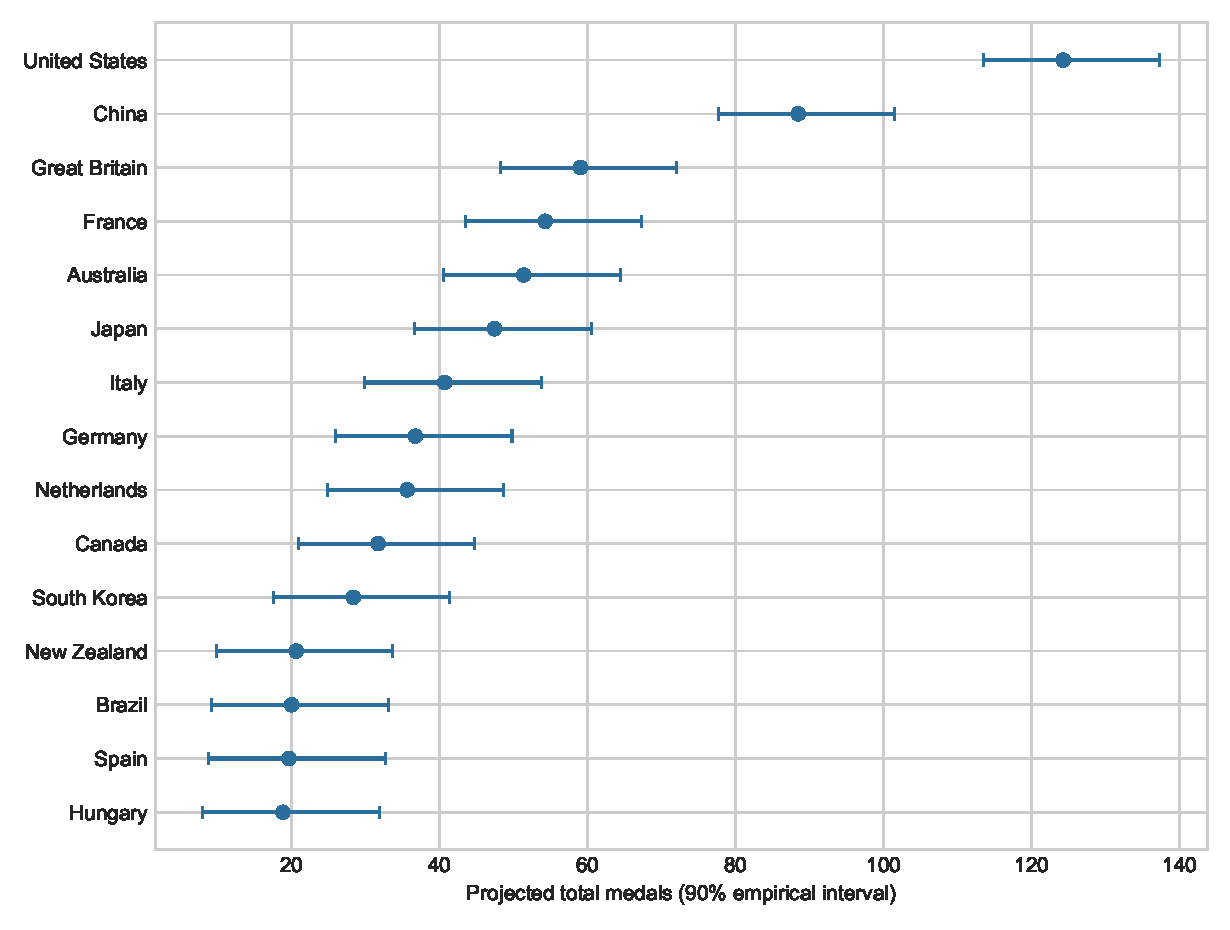
\includegraphics[width=0.78\textwidth]{figures/forecast_top15.pdf}
\caption{总奖牌点预测前 15 名及历史误差区间}
\label{fig:forecast}
\end{figure}

相对 2024 年，加拿大和德国的总牌点预测分别增加约 4.73 和 3.76 枚，日本增加约 2.44 枚。法国减少约 9.70 枚，英国减少约 5.95 枚。区间重叠仍然很大，因此这些变化用于判断方向，不应写成确定名次。美国虽然总牌点预测略低于 2024 年，金牌却因主场修正增加；总牌和金牌是分别拟合的目标，二者不要求同方向变化。

\begin{figure}[H]
\centering
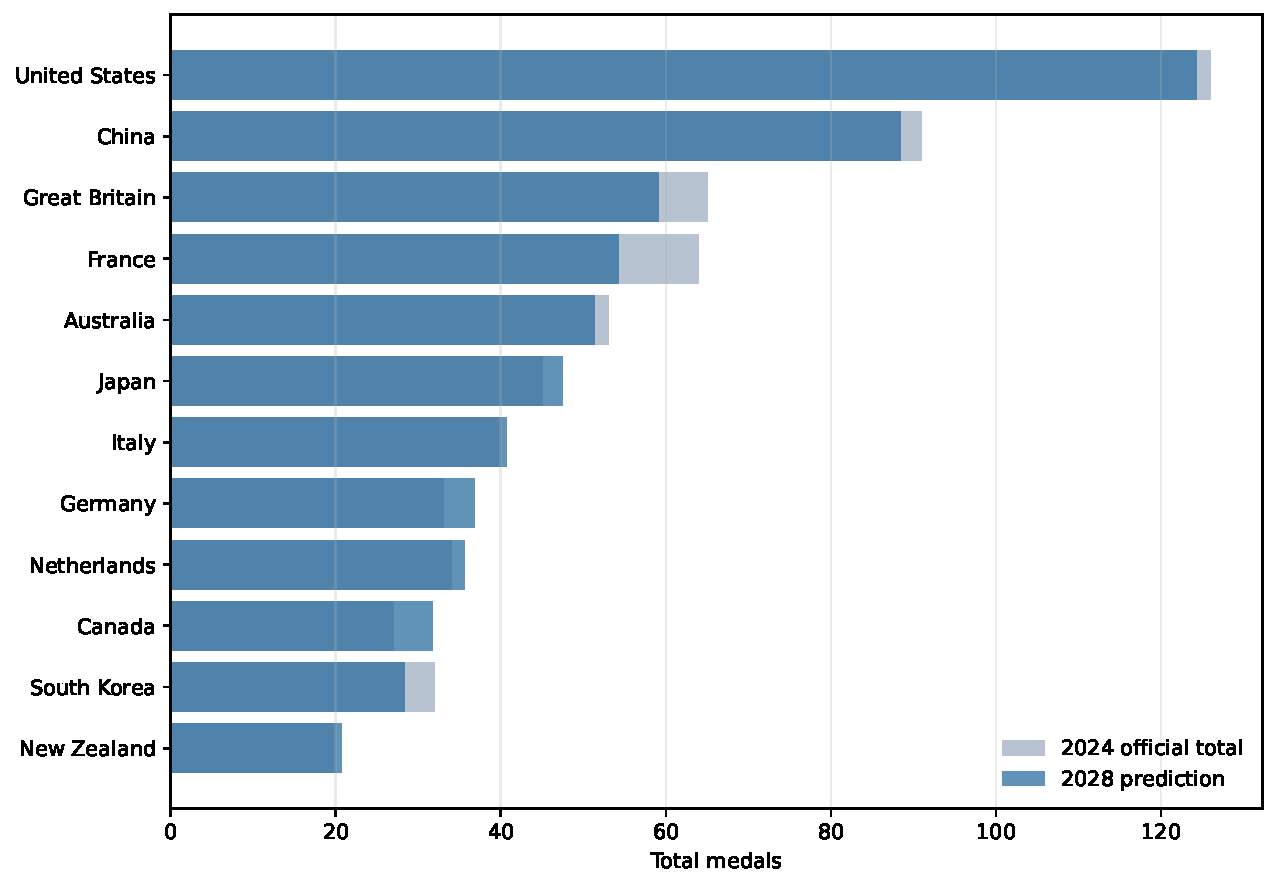
\includegraphics[width=0.82\textwidth]{figures/forecast_change.pdf}
\caption{主要国家 2028 年总牌点预测相对 2024 年的变化}
\label{fig:forecast-change}
\end{figure}

图\ref{fig:forecast-change}只展示变化方向，不把点预测差值当作确定的奖牌增量。美国的变化应分解为主场状态和模型部分；法国的下降主要来自主场状态切换；加拿大、德国和日本的上升来自历史特征、项目机会和收缩项共同作用。因为所有国家最终还经过总量校准，一国上升同时意味着其他国家的比例会发生轻微调整，图中的差值不能单独解释为“新增了同样数量的全球奖牌”。

\subsection{点预测、区间与总量校准}

模型先给出每个国家的未校准点预测，再分别乘以
\begin{equation}
c_T=\frac{1039}{\sum_i\widehat{Y}^{T,\,\mathrm{raw}}_{i,2028}},\qquad
c_G=\frac{328}{\sum_i\widehat{Y}^{G,\,\mathrm{raw}}_{i,2028}},
\end{equation}
使预测总牌和金牌与 2024 年基准项目结构下的全球总量一致。校准发生在模型输出之后，因此不会把 2028 年的国家排序反向喂给模型。随后逐国检查金牌不超过总牌，并把下界截到 0；这一步只修正不可能的数值关系，不重新优化国家排名。

区间不是对点预测附加一个相同宽度的误差条。滚动预测残差先按预测规模分箱，再取每个箱内的 5\% 和 95\% 分位数；对于样本过少的箱，回退到相邻规模箱的残差。该作法保留了“小国多为零、大国绝对误差较大”的异方差形状。以美国为例，点预测 124.27 枚，90\% 历史误差区间为 113.46--137.32；乌兹别克斯坦的区间下界接近 0，反映的是历史上低牌国家的离散程度，而不是模型认为该国一定没有奖牌。

\begin{table}[H]
\centering
\caption{若干国家的 2024--2028 总牌变化与区间宽度}
\label{tab:change-detail}
\small
\begin{tabular}{lrrrrr}
\toprule
国家 & 2024 总牌 & 2028 点预测 & 变化 & 区间下界 & 区间上界\\
\midrule
美国 & 126 & 124.27 & -1.73 & 113.46 & 137.32\\
中国 & 91 & 88.47 & -2.53 & 77.66 & 101.52\\
法国 & 64 & 54.30 & -9.70 & 43.49 & 67.35\\
加拿大 & 27 & 31.73 & 4.73 & 20.91 & 44.78\\
德国 & 33 & 36.76 & 3.76 & 25.95 & 49.81\\
日本 & 45 & 47.44 & 2.44 & 36.63 & 60.49\\
\bottomrule
\end{tabular}
\end{table}

表\ref{tab:change-detail}中的变化量只用于寻找值得解释的方向。法国的点预测仍在历史区间内，不能据此断言主场结束后必然减少 9.70 枚；同样，美国的总牌轻微下降与金牌上升并不矛盾，因为两种目标采用独立模型和独立总量校准。

\phantomsection\label{mcm-q3-start}
\subsection{项目增减的边际作用}

2028 项目列缺失后，本文不直接改动基准表，而把一项新增小项的三枚奖牌按 2016--2024 年该项目奖牌份额分配。若项目 $s$ 增加一个小项，则国家 $i$ 的总牌期望增量为
\begin{equation}
\Delta Y^T_{i,s}=3\frac{\sum_{\tau\in\{2016,2020,2024\}}M_{i,s,\tau}}
{\sum_j\sum_{\tau\in\{2016,2020,2024\}}M_{j,s,\tau}}.
\end{equation}
例如新增一个乒乓球小项，中国的边际增量约为 1.36 枚；新增一个滑板小项，日本约增加 1.13 枚；新增一个铁人三项小项，英国约增加 1.14 枚。美国的项目组合更分散：棒垒球、篮球、水上项目和田径新增一个小项，对其总牌的边际增量约为 1.00、0.75、0.71 和 0.64 枚。该计算回答“项目设置偏向谁”，并不假定主办国可以任意添加项目。

项目组合的另一个含义是风险集中。2016--2024 年只在一个项目获牌的国家，项目集中度接近 1；这里的集中度定义为各项目奖牌份额平方和。肯尼亚、牙买加和埃塞俄比亚属于这类情形。对 2020 年至少获得 3 枚奖牌的 65 个国家，集中度与 2024 相对变化绝对值的 Spearman 系数为 0.160，$p=0.203$；现有样本不足以证明集中度越高，下一届波动必然越大。因此本文把集中度作为风险提示，不把它写成已验证的预测因子。

\begin{figure}[H]
\centering
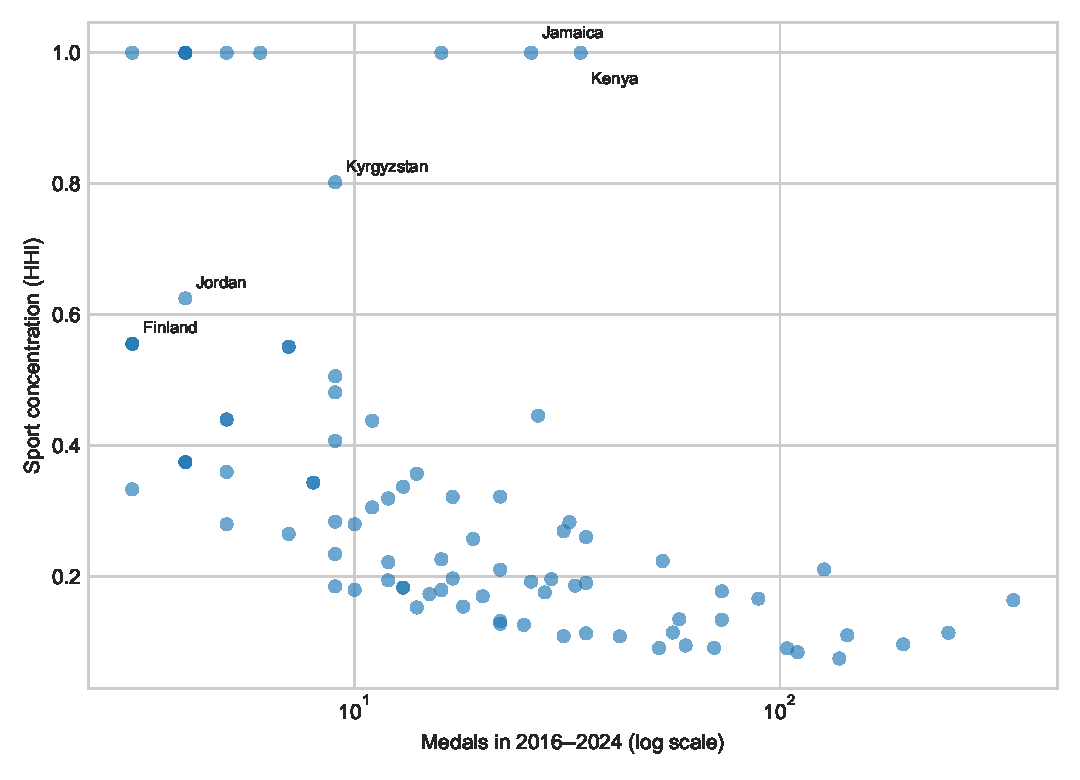
\includegraphics[width=0.78\textwidth]{figures/portfolio_concentration.pdf}
\caption{2016--2024 年项目集中度与近三届奖牌数}
\label{fig:concentration}
\end{figure}

图\ref{fig:concentration}中的横轴采用对数刻度，是因为少数国家拥有几十枚奖牌，而许多国家只有 3--5 枚。HHI=1 的点并不表示数据异常，而是该国近三届奖牌全部来自同一项目。这样的国家一旦项目被移出赛程，边际影响会比总牌相近但项目分散的国家更大；反过来，项目增加也可能集中地抬高一个国家的预测。由于本题只给到项目数量而没有完整的 2028 赛程，本文把这一观察保留为解释接口。

\begin{table}[H]
\centering
\caption{项目集中度的几个边界情形}
\label{tab:hhi-examples}
\small
\begin{tabular}{lrrl}
\toprule
国家 & 2016--2024 总牌 & HHI & 读法\\
\midrule
肯尼亚 & 34 & 1.000 & 奖牌集中在田径\\
牙买加 & 26 & 1.000 & 奖牌集中在田径\\
格林纳达 & 4 & 1.000 & 小样本单项目获牌\\
吉尔吉斯斯坦 & 9 & 0.802 & 一个项目占主导但并非全部\\
约旦 & 4 & 0.625 & 奖牌分布在少数项目\\
\bottomrule
\end{tabular}
\end{table}

\subsection{项目份额的构造与情景表}

项目边际情景使用的是同一项目内部的奖牌份额，而不是国家在全部项目中的总牌比例。对每个规范化项目，先按 2016、2020、2024 三届求和，再除以该项目所有国家的同口径奖牌总数。项目发生一次新增小项时，总共增加 3 枚可分配奖牌；若题目指定的是减少小项，则对同一份额向相反方向移动。因为份额来自过去三届，项目变化不可能把 2028 年实际结果泄漏到基准预测。

\begin{table}[H]
\centering
\caption{一项新增小项对典型国家的边际总牌增量}
\label{tab:marginal-examples}
\small
\begin{tabular}{lllrr}
\toprule
国家 & 项目 & 近三届项目奖牌份额 & 新增小项奖牌总量 & 边际增量\\
\midrule
中国 & 乒乓球 & 0.453 & 3 & 1.36\\
日本 & 滑板 & 0.377 & 3 & 1.13\\
英国 & 铁人三项 & 0.380 & 3 & 1.14\\
美国 & 棒垒球 & 0.333 & 3 & 1.00\\
美国 & 篮球 & 0.250 & 3 & 0.75\\
美国 & 水上项目 & 0.237 & 3 & 0.71\\
美国 & 田径 & 0.213 & 3 & 0.64\\
\bottomrule
\end{tabular}
\end{table}

表\ref{tab:marginal-examples}中的份额保留三位小数，边际增量由未四舍五入份额计算。中国在乒乓球上的份额高，并不意味着它能获得新增小项的全部奖牌；日本滑板的数值也会随滑板小项数量和参赛国家改变而变化。对美国而言，多个项目都出现在表中，说明它的项目组合更分散，单个项目的赛程变化不容易完全改写总牌方向。

在项目情景和国家预测之间，本文只传递一层信息：项目新增先改变该项目可分配的三枚奖牌，再把增量加到基准点预测的解释层。它不重新训练随机森林，也不改变首牌模型的样本。这样既能回答项目设置偏向谁，又避免把一个假设情景误写成新的 2028 预测表。

\subsection{多个项目变化时的组合约束}

若同时改变若干项目，只有在这些项目的小项集合互不重叠时，边际份额才可以直接相加。设新增项目集合为 $\mathcal{S}_+$、减少项目集合为 $\mathcal{S}_-$，则基准预测的解释性修正写为
\begin{equation}
\Delta Y^T_i=3\sum_{s\in\mathcal{S}_+}w_{i,s}
-3\sum_{s\in\mathcal{S}_-}w_{i,s},\qquad
w_{i,s}=\frac{\sum_{\tau\in\{2016,2020,2024\}}M_{i,s,\tau}}
{\sum_j\sum_{\tau\in\{2016,2020,2024\}}M_{j,s,\tau}}.
\end{equation}
若两个项目共享同一批小项、或项目增减改变了其他项目的参赛资格，式中份额就不再独立，必须回到项目层数据重新分配。当前附件只有历史项目列，无法判断这种联动，所以正文只报告单项目边际量，并在组合情景处保留该约束。

这也说明项目情景和国家总量校准不能机械叠加。基准预测已经把全球总牌固定为 1039 枚；项目新增情景若增加三枚奖牌，必须同时说明这三枚来自题面给出的项目总量变化，不能把它们直接加到 1039 后仍声称是同一个基准表。本文的做法是把情景结果作为“在赛程变化下的方向和份额解释”，不重新声称一张完整的全球奖牌榜。

\phantomsection\label{mcm-q1-end}
\phantomsection\label{mcm-q2-start}
\phantomsection\label{mcm-q3-end}
\section{首枚奖牌概率}

对每个预测届次，只保留此前总奖牌累计为零、且当届实际参赛的国家。输入包括上一届参赛人数、覆盖项目数、小项条目数、累计参赛届数和项目总量。Logistic 模型写为
\begin{equation}
\operatorname{logit}(p_{i,t})=\beta_0+\beta_1A_{i,t-1}
+\beta_2S_{i,t-1}+\beta_3E_{i,t-1}+\beta_4D_{i,t},
\end{equation}
其中 $D_{i,t}$ 为此前参赛届数。滚动训练中，小项条目数和参赛人数的标准化系数为正，说明更大的可进入比赛面会抬高首牌机会；参赛届数系数为负，表示长期参赛仍未获牌本身也是一条不利信息。

平衡类别训练得到的滚动平均概率为 0.281，而实际首牌率为 0.071。直接使用该输出会严重高估首牌国家数。本文保持模型的赔率排序，只调整截距使滚动平均概率回到实际发生率。校准后，以随机种子 20250814 独立重复 50000 次 Bernoulli 抽样，2028 年首牌国家数的期望为 5.08，90\% 计数区间为 2--9，至少出现一个首牌国家的概率约为 99.5\%。

校准使用赔率而不是概率的线性缩放。设滚动样本中的实际首牌率为 $\rho=0.07053$，平衡训练输出的平均概率为 $\bar p=0.28136$，则
\begin{equation}
\operatorname{odds}^{\rm cal}_{i,t}=\operatorname{odds}^{\rm raw}_{i,t}
\frac{\rho/(1-\rho)}{\bar p/(1-\bar p)},\qquad
p^{\rm cal}_{i,t}=\frac{\operatorname{odds}^{\rm cal}_{i,t}}
{1+\operatorname{odds}^{\rm cal}_{i,t}}.
\end{equation}
这个处理保留了候选国家之间的相对次序，只把整体水平拉回历史发生率。它不能解决训练样本中从未出现过的国家类型，也不能把“至少一枚奖牌”拆解成某个具体项目的概率。

\begin{table}[H]
\centering
\caption{2028 年首枚奖牌候选的校准概率}
\label{tab:first-medal-top}
\small
\begin{tabular}{lrlr}
\toprule
国家 & 校准概率 & 国家 & 校准概率\\
\midrule
黎巴嫩 & 0.305 & 南苏丹 & 0.177\\
巴勒斯坦 & 0.142 & 马绍尔群岛 & 0.141\\
安哥拉 & 0.131 & 东帝汶 & 0.125\\
几内亚比绍 & 0.122 & 基里巴斯 & 0.120\\
关岛 & 0.114 & 图瓦卢 & 0.113\\
\bottomrule
\end{tabular}
\end{table}

\subsection{首牌样本的生成与概率检验}

首牌分类的正样本定义为“该国在本届第一次出现总牌大于零”，而不是“该国本届比上一届多一枚”。因此某国一旦获得过奖牌，后续届次就从首牌训练样本中移除；它仍然可以进入总牌预测。训练特征全部取预测届次以前的参赛规模和项目面，标签则由官方奖牌榜按届次生成。这个定义避免把一个已经有奖牌基础的国家误当作首牌案例。

Logistic 模型使用中位数填补、标准化和类别平衡权重。类别平衡的目的只是让少数正样本在损失函数中不被大量零值淹没，不能据此宣称原始输出已经是校准概率。滚动预测的 Brier 分数为 0.11585；更重要的检查是平均输出概率 0.28136 与实际首牌率 0.07053 的差距。校准后再进行计数模拟，得到的期望为 5.0781 个国家，90\% 区间为 2--9。

\begin{table}[H]
\centering
\caption{首牌模型从排序到计数的检查}
\label{tab:first-medal-check}
\small
\begin{tabular}{p{4.1cm}rrp{6.0cm}}
\toprule
检查对象 & 原始值 & 校准/模拟值 & 解释\\
\midrule
滚动平均概率 & 0.28136 & 0.07053 & 校准目标为历届实际首牌率\\
滚动 Brier 分数 & 0.11585 & -- & 只用于比较概率排序，不外推为准确率\\
2028 首牌国家数期望 & -- & 5.07810 & 独立 Bernoulli 计数的均值\\
90\% 计数区间 & -- & 2--9 & 50000 次重复抽样的分位数\\
至少一个首牌概率 & -- & 0.99532 & 计数模拟中 $K\geq1$ 的比例\\
\bottomrule
\end{tabular}
\end{table}

计数模拟对每个候选国家独立抽取一次 Bernoulli 变量，未引入国家之间的奖牌竞争相关性。真实比赛中，项目资格、同一地区的参赛限制和项目赛程会使事件相关；因此 2--9 的区间是当前独立近似下的历史校准区间，而不是严格的联合分布置信区间。本文把这个限制放在计数结论附近，而不是把“99.5\%”单独作为宣传性结论。

\begin{figure}[H]
\centering
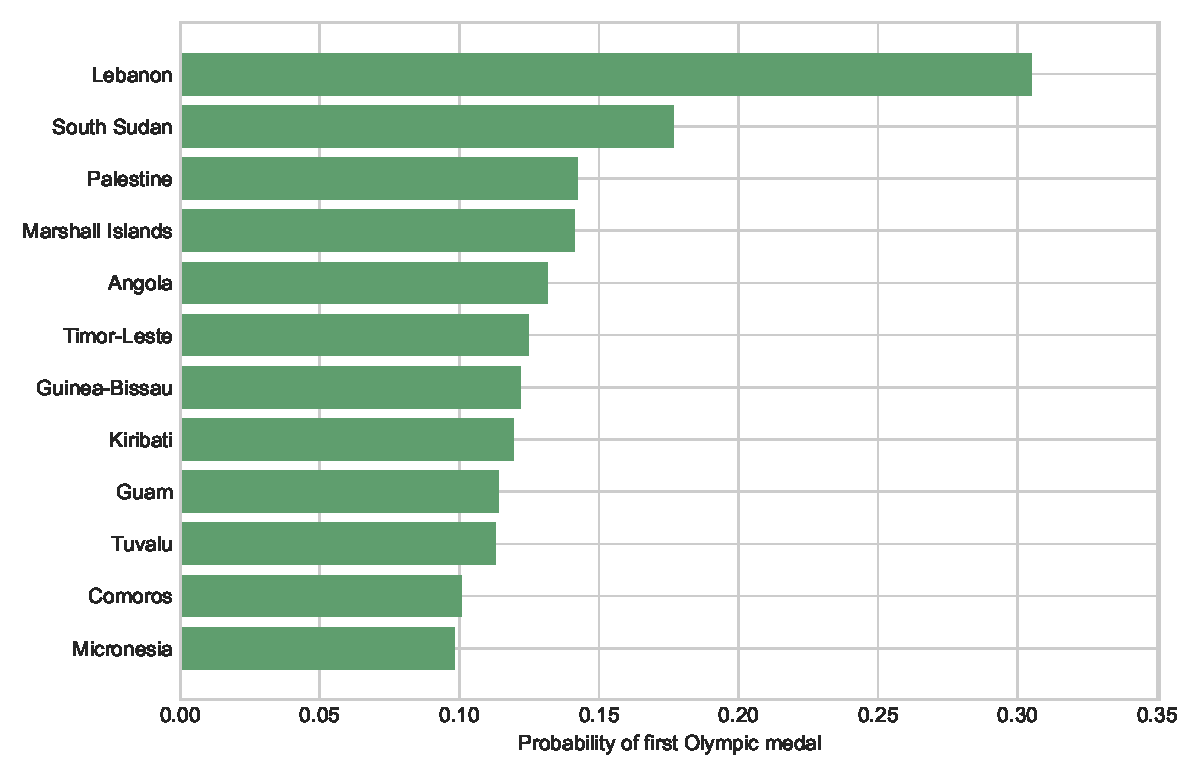
\includegraphics[width=0.76\textwidth]{figures/first_medal_probabilities.pdf}
\caption{2028 年首枚奖牌概率较高的国家}
\label{fig:firstmedal}
\end{figure}

黎巴嫩的概率约为 0.305，南苏丹为 0.177，巴勒斯坦为 0.142；其后为马绍尔群岛、安哥拉和东帝汶。这些概率反映在当前参赛规模下跨过“至少一枚”门槛的机会，不能用于预测具体项目。模型也没有把 2024 年以特殊身份参赛的 AIN 计作一个新国家。

\phantomsection\label{mcm-q2-end}
\phantomsection\label{mcm-q4-start}
\section{教练型跃升识别与投资建议}

\subsection{从项目残差中识别持续跃升}

运动员表没有教练字段。若一个国家在某项目突然增加奖牌，原因可能是运动员黄金一代、主场、项目扩容、投入增加或训练团队变化。为避免把所有跃升都命名为教练效应，先以国家--项目--届次为样本，用过去三届奖牌、参赛人数、小项条目和东道主身份拟合 Poisson 梯度提升模型，得到期望奖牌 $\widehat{M}_{i,s,t}$。标准化残差为
\begin{equation}
z_{i,s,t}=\frac{M_{i,s,t}-\widehat{M}_{i,s,t}}
{\sqrt{\widehat{M}_{i,s,t}+1}}.
\end{equation}
只有相邻两届残差都为正时，才形成一次持续跃升候选。中国体操在 2008--2012 年两届合计获得 30 枚，而模型期望约为 9.19 枚；英国自行车在 2008--2012 年两届合计 26 枚，期望约为 13.66 枚；荷兰田径在 2020--2024 年合计 14 枚，期望约为 6.02 枚。它们说明模型未解释的项目能力发生了持续变化，下一步应外接教练任职、训练投入和运动员代际数据，而不是据此直接认定某位教练贡献了残差中的全部奖牌。

\begin{figure}[H]
\centering
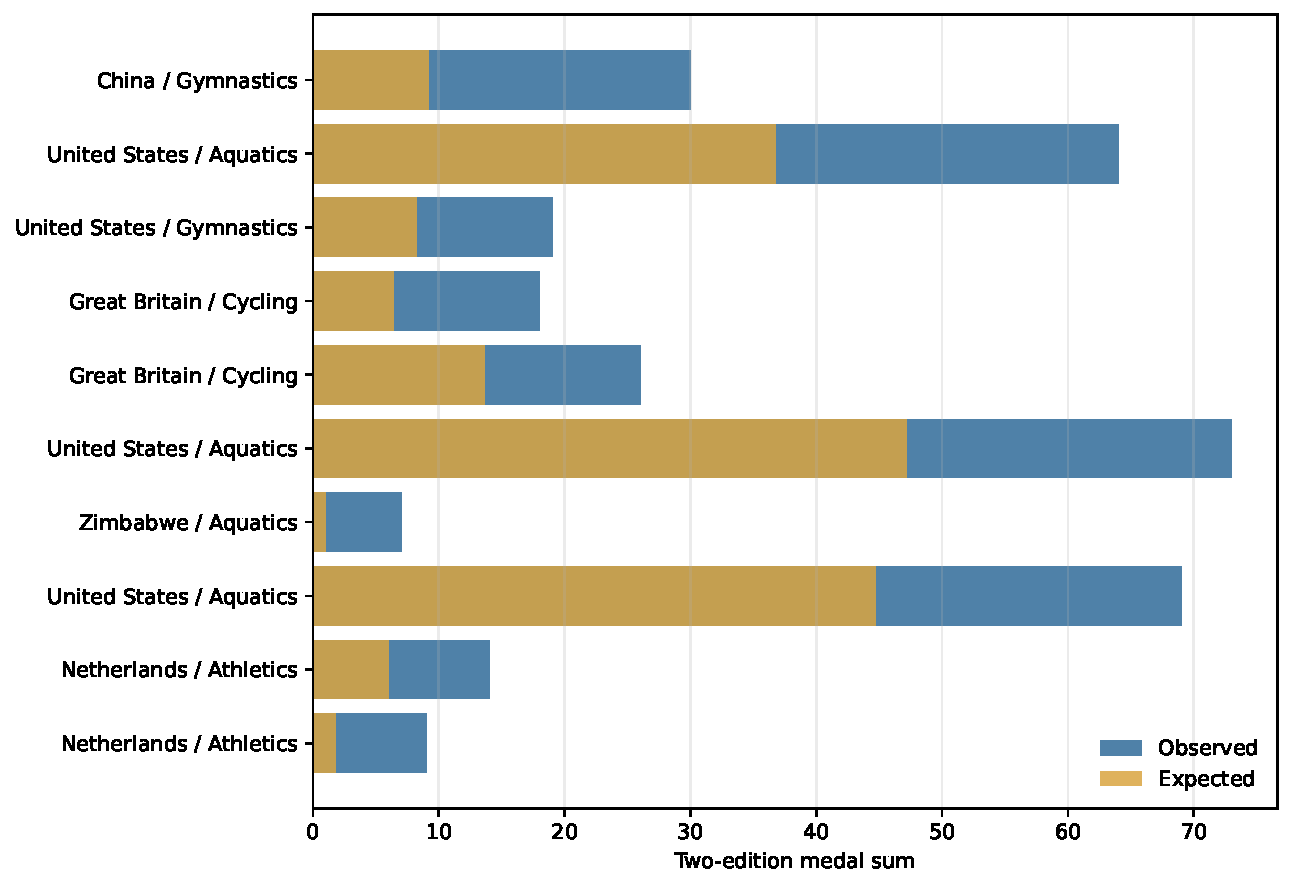
\includegraphics[width=0.80\textwidth]{figures/coach_episode_comparison.pdf}
\caption{持续正残差片段的观测奖牌与模型期望}
\label{fig:coach-episodes}
\end{figure}

图\ref{fig:coach-episodes}中的柱高是两届合计值，候选筛选并不依赖某一个异常年份。以中国体操为例，先在 2008 年出现正残差，2012 年仍保持正残差，才被记录为一个片段；若第二届回到模型期望附近，则该片段不会进入候选表。英国自行车和荷兰田径的候选也按同一规则生成。这个规则留下了一个可供外部资料核对的时间窗口，而不是把“教练”当成数据中已经存在的字段。

\begin{table}[H]
\centering
\caption{持续正残差候选的观测与模型期望}
\label{tab:coach-episodes}
\small
\begin{tabular}{llrrrr}
\toprule
国家 & 项目 & 时间段 & 观测奖牌 & 模型期望 & 超额/枚\\
\midrule
中国 & 体操 & 2008--2012 & 30 & 9.19 & 20.81\\
英国 & 自行车 & 2008--2012 & 26 & 13.66 & 12.34\\
荷兰 & 田径 & 2020--2024 & 14 & 6.02 & 7.98\\
牙买加 & 田径 & 2008--2012 & 21 & 9.70 & 11.30\\
津巴布韦 & 水上项目 & 2004--2008 & 7 & 0.99 & 6.01\\
\bottomrule
\end{tabular}
\end{table}

表中的“超额”只是一种筛选分数，不能当作可分配给教练的奖牌数。项目模型已经控制了上届奖牌、运动员数、小项条目和主场状态，但没有控制运动员年龄结构、伤病、国家队选拔和训练投入，因此剩余部分仍可能来自这些未观测因素。候选名单的用途是缩小后续资料核查范围。

\subsection{三个投资情景}

投资建议使用另一个更保守的接口。固定近两届平均参赛人数，把项目奖牌/运动员转化率提高到同项目、且参赛人数不少于 5 人的国家上四分位，得到有限增量
\begin{equation}
G_{i,s}=A_{i,s}\max\{0,Q_{0.75,s}-c_{i,s}\},
\end{equation}
并将单项目增量截在 5 枚以内。该情景假定投入主要改善训练转化，而不立即扩大代表团规模。

\begin{table}[H]
\centering
\caption{建议关注的三个国家--项目情景}
\label{tab:coach}
\begin{tabular}{llrrr}
\toprule
国家 & 项目 & 近两届平均运动员数 & 当前转化率 & 估计增量/枚\\
\midrule
德国 & 田径 & 88.0 & 0.0398 & 4.10\\
西班牙 & 水上项目 & 52.5 & 0.0286 & 4.07\\
埃及 & 击剑 & 17.5 & 0.0286 & 3.56\\
\bottomrule
\end{tabular}
\end{table}

德国田径的参赛面已经很大，问题在于奖牌转化率低于同项目上四分位；若教练团队改善决赛转化与多小项协同，增量空间较大。西班牙水上项目也具备较大的运动员基数，适合以专项教练和分项训练提高转化。埃及击剑近两届平均派出 17.5 名运动员，当前转化率约为 0.0286；若提升至同项目上四分位，情景增量约 3.56 枚。三项结果均是资源配置上限附近的可观测差距，不是承诺值；若外部履历不能证明教练变更发生在跃升以前，应撤回“伟大教练”解释，仅保留项目能力投资建议。

\subsection{投资情景的筛选顺序}

投资情景不是从所有国家--项目组合中直接取增量最大的三项。代码先保留近两届总牌为 1--40 枚、当届运动员人数不少于 8 人的国家，再在项目层要求近两届平均运动员数不少于 5 人。这样做有两个现实含义：过大的传统强国不因为基数而占满候选，只有一名运动员的项目也不因一次偶然奖牌而进入建议表。

对保留下来的组合，当前转化率定义为近两届项目奖牌数除以近两届运动员数；比较组是同一项目中运动员人数至少为 5 的国家，$Q_{0.75,s}$由这些转化率的上四分位数得到。增量先按 $A_{i,s}(Q_{0.75,s}-c_{i,s})_+$计算，再截断为 5 枚。这个截断不是统计估计，而是情景的预算上限，避免一个较大的代表团把小数差距直接放大成不受约束的几十枚奖牌。

\begin{table}[H]
\centering
\caption{三个投资候选的筛选记录}
\label{tab:investment-screen}
\small
\begin{tabular}{llrrrr}
\toprule
国家 & 项目 & 近两届平均运动员数 & 当前转化率 & 上四分位目标 & 情景增量\\
\midrule
德国 & 田径 & 88.0 & 0.0398 & 0.0864 & 4.10\\
西班牙 & 水上项目 & 52.5 & 0.0286 & 0.1062 & 4.07\\
埃及 & 击剑 & 17.5 & 0.0286 & 0.2320 & 3.56\\
\bottomrule
\end{tabular}
\end{table}

这里的目标转化率来自项目横截面的分位数，并不声称德国、 西班牙或埃及可以在一届内达到该分位数。若把运动员人数也作为投资对象，情景会同时改变代表团规模和项目份额，当前数据无法把两种作用分开。因而本文只固定近两届平均人数，解释为“在现有参赛面上改善转化”的上限。

三个候选还需要一个外部顺序：先核对项目在 2028 年是否仍保留，再核对教练任职时间是否早于残差跃升，最后才讨论投入规模。若任职时间不吻合，项目仍可以作为能力缺口，但“教练型”标签应从结论中删除。这个退出条件使投资建议不会反过来替残差寻找一个事后故事。

\phantomsection\label{mcm-q4-end}
\section{模型检验与敏感性}

\subsection{目标、代码和结果的闭合检查}

国家级目标由官方奖牌表逐届映射到运动员表的 NOC。2024 年韩国、捷克、伊朗、土耳其、香港等名称经过映射后分别恢复为 32、5、12、8、4 枚总牌；运动员表有奖牌而官方目标为零的普通国家数量为 0。2028 点预测校准后，各国总牌之和为 1039，金牌之和为 328，且逐国满足金牌不超过总牌。团队项目只在项目归属表中去重，不替代官方国家汇总。

\subsection{模型权重}

收缩权重从 0.25 和 0.50 两个候选中选择。金牌预测中，东道主基线、随机森林、25\% 森林和 50\% 森林的滚动 MAE 分别为 0.655、0.679、0.634 和 0.627；树模型并非单独最好，只有与基线组合后误差下降。总牌预测的对应 MAE 为 1.474、1.537、1.444 和 1.441。50\% 方案在全体国家和前 20 名两个口径下都略优于 25\% 方案，因此最终采用等权收缩，而不是按模型复杂度作选择。

\begin{table}[H]
\centering
\caption{候选模型的全期平均 MAE}
\label{tab:model-comparison}
\small
\begin{tabular}{lrrrr}
\toprule
模型 & 总牌 MAE & 总牌前20名 MAE & 金牌 MAE & 解释角色\\
\midrule
上一届持续性 & 1.468 & 7.450 & 0.671 & 最简基线\\
东道主修正 & 1.474 & 7.422 & 0.655 & 结构基线\\
随机森林 & 1.537 & 7.715 & 0.679 & 非线性补充\\
Poisson 梯度提升 & 1.555 & 8.520 & 0.699 & 计数模型对照\\
25\% 森林收缩 & 1.444 & 7.189 & 0.634 & 小幅引入树模型\\
50\% 森林收缩 & 1.441 & 7.118 & 0.627 & 最终方案\\
\bottomrule
\end{tabular}
\end{table}

表\ref{tab:model-comparison}中前 20 名平均误差保留三位小数，实际选择使用未四舍五入的值。对数岭回归的总牌 MAE 为 3.226、金牌 MAE 为 1.020，未进入上表的候选层；它作为线性可解释参照保留在 \path{rolling_validation.csv} 中。这样做的目的不是证明岭回归“错误”，而是说明在长尾和强国同时存在的目标分布下，单一对数线性关系承担不了全部变化。

\subsection{主场状态的局部检验}

主场修正的作用可以从三个状态比较：普通届次使用 $B^q_{i,t}$，主办国使用 $B^q_{i,t}+b^q_t$，离开主场的国家使用 $B^q_{i,t}-b^q_t$。由于 $b^q_t$ 是训练窗口中的中位残差，主场修正不随单个国家的历史牌数成比例增长；同一个修正量施加到小国和强国，作用的绝对大小相同，随后再由随机森林部分区分两者。

这一设置带来一个需要主动说明的结果：美国的总牌点预测并没有因为主场身份自动超过 2024 年，而金牌点预测却出现上升。总牌与金牌分别校准到 1039 和 328 枚，且两套模型的残差分布不同，因而不能从“主场加成”推出两个目标必然同向。法国的回落则是同一状态变量从 $H_{i,t-1}=1$ 变为 $H_{i,t}=0$ 的结果。我们把这两种状态切换都保留在结果解释中，而不是只报告最后的国家排序。

\subsection{结果文件的逐层回查}

一次完整重算依次生成特征面板、滚动验证、点预测与区间、首牌概率、跃升片段和投资情景。各层文件与检查接口见表\ref{tab:result-interface}。图形脚本只读取这些结果文件，不再独立重算一套数字。

\begin{table}[H]
\centering
\caption{从数据到结论的结果接口}
\label{tab:result-interface}
\small
\begin{tabularx}{\textwidth}{p{4.0cm}p{4.2cm}X}
\toprule
输出层 & 主要文件 & 本文检查的接口\\
\midrule
特征层 & \path{model_panel.csv} & 目标届次以前的滞后变量、主场状态和项目机会\\
验证层 & \path{rolling_validation.csv} & 2008--2024 五个验证点、MAE/RMSE/前20名 MAE\\
预测层 & \path{forecast_2028.csv} & 点预测、经验区间、总牌和金牌校准\\
分类层 & \path{first_medal_probabilities.csv} & 校准概率、50000 次计数模拟所需输入\\
项目层 & \path{sport_event_marginal_shares.csv} & 一项新增小项的份额分配\\
跃升层 & \path{coach_like_episodes.csv} & 相邻两届正残差和模型期望\\
\bottomrule
\end{tabularx}
\end{table}

表\ref{tab:result-interface}是复现检查清单而不是正文的八段模板。若只替换 \texttt{forecast\_2028.csv} 而不重跑滚动验证，旧的模型选择仍会留在正文；若只更新图形而不核对表格，图表和文字也可能来自不同版本。因此结果同步脚本同时检查来源文件哈希和正文中的关键数字，发现源文件改变时先暂停润色。

\subsection{大误差片段的解释边界}

滚动预测中有几次绝对误差远大于平均值。表\ref{tab:large-residuals}列出最终收缩方案的部分片段，目的是说明平均 MAE 没有掩盖数据 regime 的变化，而不是把每个片段都改造成新的模型。2020 年 ROC 的官方总牌为 71 枚，而上一届同口径历史和可用参赛特征不足以预见这一特殊代表团的集中表现；2008 年中国和俄罗斯的相反方向误差，则与两国在主场周期和项目结构中的大幅转移同时出现。

\begin{table}[H]
\centering
\caption{总牌预测中的典型大残差片段}
\label{tab:large-residuals}
\small
\begin{tabular}{lrrrrr}
\toprule
届次 & NOC & 实际总牌 & 预测总牌 & 预测--实际 & 解释侧重点\\
\midrule
2020 & ROC & 71 & 0.15 & -70.85 & 特殊代表团口径\\
2008 & 中国 & 100 & 72.56 & -27.44 & 主场与项目跃升\\
2008 & 俄罗斯 & 60 & 87.10 & 27.10 & 前期成绩惯性\\
2016 & 中国 & 70 & 92.26 & 22.26 & 结构变化未被完全吸收\\
2024 & 法国 & 64 & 41.88 & -22.12 & 主场增量的局部性\\
\bottomrule
\end{tabular}
\end{table}

这些片段直接决定了本文的两个边界。第一，区间用滚动残差分位数而不是模型标准误，因为特殊代表团和主场跃升并不满足同方差假设。第二，模型评价不能只看强国的某一次误差；它还要同时报告长尾国家的总体 MAE，否则一个被 ROC 拉高的残差会主导对模型的判断。表\ref{tab:rolling-detail}与表\ref{tab:large-residuals}配合使用，分别回答“整体表现怎样”和“异常来自哪里”。

\subsection{项目和首牌结果的边界}

项目情景每增加一个小项，只重新分配该项目的三枚奖牌，不改变其他项目。中国乒乓球、日本滑板和英国铁人三项的边际增量分别约为 1.36、1.13 和 1.14 枚；若新增项目并未采用这些国家近期优势相同的竞赛设置，实际增量会偏离该值。

首牌模型最敏感的是概率校准。未校准时，候选国家平均概率为 0.281，明显高于滚动验证中的实际 0.071；校准后首牌期望为 5.08。若取消类别平衡而直接拟合，候选排序会更多集中在大型代表团，少数潜在国家的召回下降。因此本文保留平衡训练用于排序，但不允许其原始概率直接进入数量结论。

\subsection{四个问题之间的数据传递}

四个问题虽然共享历史数据，但每一问只接收上一层确实产生的量。国家预测把官方奖牌榜压缩为国家--届次目标；项目情景从运动员记录得到国家--项目份额；首牌模型从国家是否曾获牌构造二元标签；教练型跃升则在国家--项目--届次上使用国家预测中没有用到的项目奖牌。表\ref{tab:question-interface}列出了这些接口，防止一个问题的结果未经说明地变成另一个问题的特征。

\begin{table}[H]
\centering
\caption{分问题之间的变量传递关系}
\label{tab:question-interface}
\small
\begin{tabularx}{\textwidth}{p{2.4cm}p{4.2cm}p{4.5cm}X}
\toprule
问题 & 样本单位 & 从前一层接收的量 & 新增处理\\
\midrule
问题一 & 国家--届次 & 官方总牌、金牌、参赛规模 & 16 个滞后特征、主场基线、滚动验证\\
问题二 & 未获牌国家--届次 & 参赛规模与项目面 & Logistic 排序、赔率校准、计数模拟\\
问题三 & 国家--项目 & 2016--2024 项目奖牌份额 & 单项目新增/减少小项的边际情景\\
问题四 & 国家--项目--届次 & 项目奖牌、参赛人数、主场状态 & Poisson 梯度提升、连续正残差、转化率情景\\
\bottomrule
\end{tabularx}
\end{table}

问题二没有接收问题一的点预测，是因为“已有奖牌国家的总牌数”与“尚未获牌国家第一次越过零点”不是同一目标。问题三也没有把项目边际增量重新加回问题一的全球总量，而是保留为赛程变化下的局部解释。问题四的残差模型使用项目奖牌，而非把问题一的国家总牌拆分后再拟合，这避免团队小项去重规则在两个层面重复应用。

\subsection{敏感性只改变一个接口}

本文的敏感性比较遵循“一次只动一处”。权重敏感性只改变基线和随机森林的混合系数，项目敏感性只改变新增小项的份额，概率敏感性只比较校准前后的首牌计数。主场加成、全球总量和国家名称映射保持固定，因而可以判断输出变化究竟来自哪一个假设。

例如把收缩权重从 0.25 调到 0.50 时，总牌平均 MAE 从 1.4435 降到 1.4408，金牌平均 MAE 从 0.6341 降到 0.6266；这两个改变量都来自滚动验证，不是 2028 点预测反推。首牌部分从原始平均概率 0.2814 调到历史率 0.0705 后，期望首牌国家数从未经校准的高估状态回到 5.0781。项目部分则不重新拟合总牌模型，只观察式中的 $w_{i,s}$如何改变边际增量。

\begin{table}[H]
\centering
\caption{单接口敏感性检查}
\label{tab:sensitivity-single}
\small
\begin{tabularx}{\textwidth}{p{3.5cm}p{3.1cm}p{3.1cm}X}
\toprule
改变的接口 & 基准 & 改变后 & 保持不变的量\\
\midrule
收缩权重 & 0.25 森林 & 0.50 森林 & 训练窗口、目标总量、随机种子\\
首牌概率 & 原始均值 0.2814 & 校准均值 0.0705 & 候选排序、特征和标签\\
项目数量 & 2024 结构 & 单项 $+1$ 或 $-1$ & 国家级点预测、首牌样本\\
跃升条件 & 单届正残差 & 相邻两届正残差 & 项目模型和超参数\\
\bottomrule
\end{tabularx}
\end{table}

敏感性结果没有用来挑选一个最漂亮的数字，而是用来识别结论的稳定部分：美国、中国位于前列、首牌候选集中在参赛规模较小的国家、项目边际量随近期份额变化，这些方向在接口微调后仍可解释；具体的 124.27、5.08 和 4.10 则必须连同口径和区间一起报告。

\section{模型评价与进一步数据}

\subsection{复现与人工核对的分工}

本文把“脚本能重跑”和“正文能解释”分成两条检查线。脚本线从四张官方 CSV 重新生成国家面板、项目去重表和结果文件；正文线则按问题逐项回到题面、公式、表格和边界。脚本线通过只说明同一组输入能得到同一组数，不能替代人工判断变量是否用错；正文线读懂一个数字的来路，也不能替代重新计算。

\begin{table}[H]
\centering
\caption{结果交付前的两条核对线}
\label{tab:manual-recheck}
\small
\begin{tabularx}{\textwidth}{p{3.2cm}p{5.1cm}p{5.3cm}}
\toprule
核对线 & 脚本检查 & 人工需要回答的问题\\
\midrule
数据层 & 行数、年份范围、NOC 映射、团队奖牌去重 & 这一行到底代表运动员、项目奖牌还是国家目标？\\
模型层 & 滚动切分、随机种子、超参数和输出列 & 首个模型名之前是否已经交代了题面关系和取舍？\\
结果层 & 总牌 1039、金牌 328、金牌不超过总牌 & 这个数字是原始输出、校准值还是情景增量？\\
图表层 & 文件存在、标签可引用、数值来自当前结果文件 & 图或表改变了哪一个判断，而不是只占了版面？\\
边界层 & 覆盖清单八类接口齐全 & 结论是否越过了数据能够支持的范围？\\
\bottomrule
\end{tabularx}
\end{table}

人工核对从摘要开始，而不是等到最后一页。摘要中的 124.27、88.47、5.08 和 4.10 分别在正文表格、首牌模拟和投资情景中找到对应位置；若结果源文件更新，先检查这些关键字面量，再检查结论段和附录入口。国家名称按当前输出表回读，不能因为中文译名顺手而把 NOC 代码换成另一届的名称。图\ref{fig:forecast}、图\ref{fig:firstmedal}和图\ref{fig:coach-episodes}只在对应结果文件生成后才进入正文。

对公式的人工复核只做三件事：检查新变量是否在符号表或附近定义，检查单位和求和范围是否与代码一致，检查公式后的解释有没有把局部量说成全球量。比如式\eqref{eq:opportunity}中的 $M_{i,s,\tau}$是去重后的项目奖牌，不是运动员获牌行；式中的三届窗口也不能在文字中改成“近四届”。同样，首牌概率的 90\% 区间来自模拟计数，不能在表格标题中写成每个国家的概率置信区间。

结果解释还要与模型选择的时间顺序相符。2028 年没有真实结果，因而只能报告点预测、历史误差区间和项目情景；模型优劣来自 2008--2024 年的滚动验证。若把 2028 的美国和中国排名写成“验证表明”，就是把预测和验证混在了一起。本文在结论中使用“位于前列”“方向”“候选”等有限词，是因为区间重叠和题面缺失仍然存在；这些词不是为了弱化结果，而是对证据范围的准确标记。

\subsection{从审计输出到正文取舍}

正式稿的审计结果只报告缺口，不自动改写正文。逐问覆盖清单若发现某一问缺少变量或检验，先回到代码和数据寻找真实接口；如果该接口确实不存在，就在边界处降低结论强度，并在清单中记录 waiver。比如 2028 项目列缺失不是通过增加一段项目背景来“补齐”，而是明确把基准项目结构固定为 2024 年，把新增项目放到情景公式中。教练字段缺失也不通过补写教练姓名解决，而是把残差片段变成外部资料核查名单。

篇幅扩展同样遵循这一取舍。有效增量来自去重键、滞后特征、滚动切分、残差分位数、项目份额、赔率校准和结果接口；算法教材、重复题面和逐格复述不进入正文。这样即使把完整代码和全量结果移到附录，正文仍然保留每个分问从数据到判断的必要路径，读者可以沿着表和公式复算主要数字。

本文的主要优点不在于使用了多种算法，而在于将三个容易混淆的口径分开：官方奖牌表负责国家目标，运动员表负责参赛规模和项目归属，项目缺失列通过情景接口处理。滚动验证使 2028 年没有参与模型选择；复杂模型若不能胜过上一届基线，就只以收缩项进入最终预测。首牌概率也没有把平衡分类器的原始输出当作真实概率。

局限同样明确。第一，2028 项目表缺失，当前点预测仍是 2024 项目结构下的基准，新增项目的相互作用没有进入总表。第二，国家名称虽已逐届映射，但国家分裂、合并和特殊代表团的历史连续性仍只能按 NOC 口径处理。第三，奖牌区间来自历史残差分位数；强国样本少，区间较宽，不能解释为某一国家自身参数的不确定性。第四，附件没有人口、经济投入、运动员当前状态、教练履历和任期，“教练型跃升”只能产生外部核查名单。

若补充 2028 正式项目表，式\eqref{eq:opportunity}和全球总量校准可以直接重算；若补充教练任职年份、训练投入和运动员年龄结构，可把候选跃升前后的项目与相似国家组成对照组，采用事件研究或合成控制估计净效应。当前结果停在附件能够支持的位置。

\subsection{后续扩展的先后顺序}

若要把这份盲测稿推进到正式研究，改进顺序应由误差源决定，而不是继续堆叠算法。第一优先是补齐 2028 年正式项目表，重新计算 $N_{s,t}$ 和全球总量；这一项直接影响基线缩放与项目边际情景。第二优先是把国家名称映射扩展为可审计的历史实体表，对分裂、合并和特殊代表团给出连续性标记，而不是只依赖 NOC 字符串。第三优先是补充运动员年龄、伤病、投入和教练任职年份，将“参赛规模代理”与真正的竞技状态分开。

模型层面可以在上述数据补齐后比较分层计数模型与当前收缩模型：国家层先估计奖牌总量，项目层再分配到小项，并用共享的全球总量约束两层输出。首牌问题可以加入项目资格和地区配额的联合模拟，替代当前独立 Bernoulli 近似；教练型跃升则可以围绕任职年份构造事件窗口，并选择相似国家做合成控制。只有这些变量实际出现，复杂模型才有新的识别对象；在当前附件上继续增加黑箱模型，只会让结果文件变多而不改变结论边界。

这一路线也保留了本文已经验证的接口：官方奖牌榜仍是国家目标，运动员表仍需团队小项去重，项目表仍通过份额进入情景，滚动验证仍按届次向前。未来版本若改动其中任一接口，必须同时更新结果源哈希、正文数字、覆盖清单和编译审计，不能只替换一张预测图。

\section{结论}

在 2024 项目结构基准下，美国和中国仍位于 2028 奖牌榜前列。模型给出的美国总牌、金牌点预测为 124.27 和 43.79，中国为 88.47 和 38.86。法国退出主场周期后出现较明显回落；加拿大、德国和日本的总牌数有小幅改善。尚未获牌国家中，2028 年预计约有 5.08 个取得首牌，90\% 计数区间为 2--9 个。

项目设置的作用取决于一国近期奖牌结构。新增乒乓球小项对中国、滑板小项对日本、铁人三项对英国的边际影响较大；美国的优势分布在多个项目。历史项目残差可以定位持续跃升，却不能在没有教练数据时完成因果归因。德国田径、西班牙水上项目和埃及击剑具有较大的转化率提升空间，适合作为进一步核查和投资的三个对象。

\phantomsection\label{mcm-body-end}
\begin{thebibliography}{9}
\bibitem{comap-problem} COMAP. 2025 MCM Problem C: Models for Olympic Medal Tables, 2025.
\bibitem{comap-data} COMAP. 2025 Problem C Data: medal counts, athletes, hosts and programs, 2025.
\bibitem{rf} Breiman L. Random Forests. \emph{Machine Learning}, 2001, 45: 5--32.
\bibitem{logit} Hosmer D W, Lemeshow S, Sturdivant R X. \emph{Applied Logistic Regression}. Wiley, 2013.
\end{thebibliography}

\appendix
\section{复现说明}

入口脚本为 \texttt{analysis/model\_pipeline.py}。脚本读取四张官方 CSV，生成滚动验证、2028 预测、首牌概率、项目边际份额、教练型残差和图形。随机森林与 Monte Carlo 计数统一使用种子 20250814。主要结果文件位于 \texttt{analysis/results/}：
\begin{itemize}
\item \texttt{rolling\_validation.csv}：逐届、逐模型误差；
\item \texttt{forecast\_2028.csv}：各国点预测与区间；
\item \texttt{first\_medal\_probabilities.csv}：首牌候选；
\item \texttt{coach\_like\_episodes.csv}：持续正残差片段；
\item \texttt{coach\_investment\_candidates.csv}：项目投资情景；
\item \texttt{summary.json}：模型选择和数据边界。
\end{itemize}

\section{人工智能工具使用说明}

本盲测使用生成式人工智能辅助读取本地题面、编写分析脚本、组织 LaTeX 初稿和执行一致性检查。所有数值均由随附脚本从题目数据重新计算；国家键映射、团队项目去重、模型选择、概率校准、预测总量和公式--代码接口经过逐项复核。文中未使用同题解答或获奖论文作为建模来源。正式参赛时仍需按当届 COMAP 规则提交完整的 AI Use Report，并由队员对模型、代码、引用和文字承担最终责任。

\end{document}
